%!TEX root = ../../csuthesis_main.tex
\chapter{类脑视觉模型理论基础}

\section{人类视觉系统启发机制}

\subsection{视觉皮层的层级结构与功能分区}

视觉系统是人类的感知系统中最复杂的信息处理通路之一,它具备分层处理、反馈调节与注意力引导等关键能力。类脑视觉模型的设计正是受到这些神经机制的启发,从结构与功能层面尝试模拟大脑的视觉加工过程。

人类的大脑的视觉信息主要沿腹侧通路(ventral stream)由初级视觉皮层(V1)向高级皮层区域(如V4、IT)逐级传递。V1主要负责边缘、方向和空间频率等低级特征的提取,而V2就在此基础上构建出更加复杂的几何形状与边缘连接关系。高级视觉皮层V4在色彩与中等复杂度图形识别方面具有关键作用,最终的高层抽象与对象识别功能则在颞下皮层区(IT)实现,这个区域神经元对类别和语义具有一定选择性。

\begin{figure}[hbt]
	\centering
	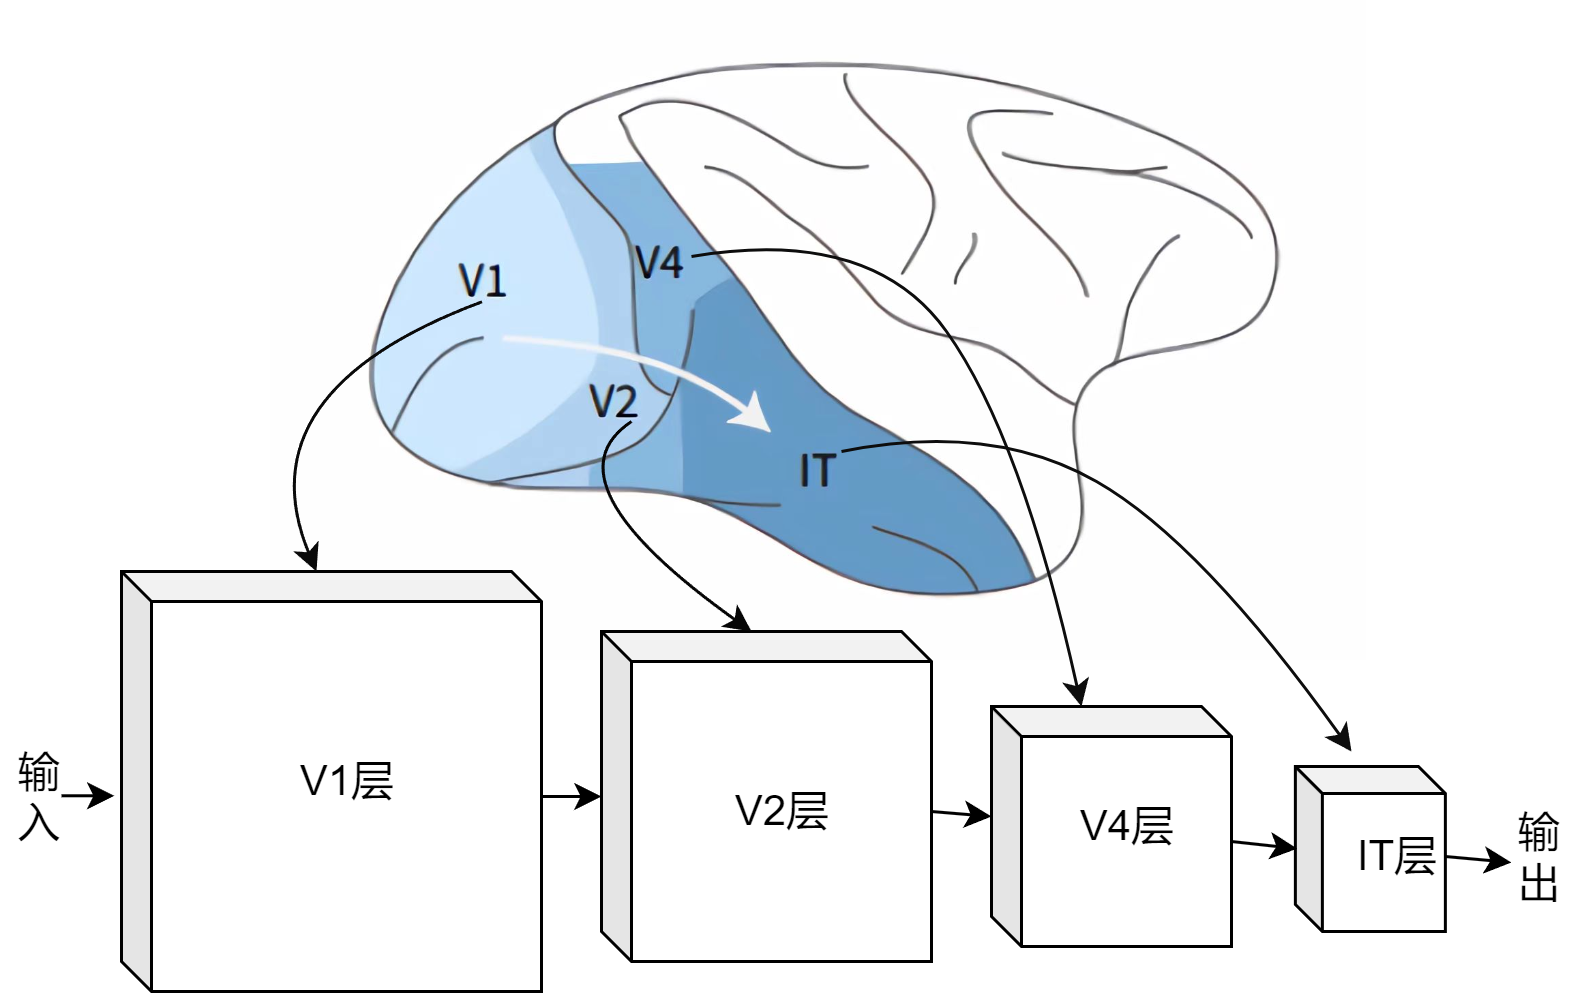
\includegraphics[width=0.3\linewidth]{brain.png}
	\caption{脑视觉区域}
	\label{f.example}
\end{figure}

CORnet模型家族就是参考这种层级顺序设定模型结构的,自底向上包括V1、V2、V4和IT四个模块,每个模块之间通过标准卷积或者残差连接实现的信息传递。CORnet模型的这种分区结构对比传统的CNN更加具有神经结构对应性,是构建类脑模型的重要基础。

\subsection{反馈调节与时间动态特性}

与传统的深度网络中固定的一次性前向传递不同,生物视觉系统中的信息加工具有强烈的动态性。视觉皮层各层之间存在着大量回馈通路(feedback connection),例如IT至V4、V4至V2甚至反向连接至V1。这些通路不仅用于错误纠正和特征重构,也参与图像完成、目标保持等高级认知活动。

这种反馈机制在在识别存在遮挡或者模糊等不完全输入的图像上显得尤其重要。例如,当一个物体的一部分被其他物体遮挡时,V1的初始响应可能不完整,但通过高层区域(如IT)反馈下行信息后,初级区域就可以对遮挡边缘做出更加准确的补全预测。这种时间上的迭代更新被视为大脑“渐进式认知”的体现。

在CORnet-S模型的设计中就引入了时间步结构,尝试模拟反馈机制产生的表征动态。不同时间步的重复计算可视为皮层对视觉输入的多次内循环处理,为建模时间延迟与稳定表征提供了基础。

\subsection{注意力机制在神经计算中的作用}

视觉注意力机制是大脑主动调节资源分配的重要方式。研究显示,顶叶皮层(如LIP区)与额叶区域参与注意力的空间选择与通道抑制,对早期视觉区域的信息通量具有显著影响。在目标搜索、快速反应等任务中,注意力可以显著增强对特定图像区域或通道的神经响应,提高识别效率与准确率。

受此启发,人工神经网络中逐步引入了注意力模块。SE(Squeeze-and-Excitation)机制通过全局平均池化压缩特征信息,并学习通道之间的响应权重,实质上模拟了神经系统中对显著特征通道的强化作用。CBAM进一步扩展了空间维度注意力,使模型能同时选择“看哪里”和“看什么”。

尽管注意力机制在模型准确率方面已有显著提升,其对类脑相似性的影响仍缺乏系统研究。部分研究发现,注意力机制在提升模型表现的同时,可能打破与大脑层级响应之间的对应关系,这也是本文后续章节关注的重点之一。

\section{CORnet模型架构解析}

\subsection{CORnet-Z与CORnet-S模型结构比较}

CORnet(Core Object Recognition network)系列模型由MIT的Kubilius等人提出,旨在构建结构与功能均尽量贴近灵长类视觉系统的深度神经网络。该模型家族的命名灵感来源于“大脑核心视觉识别能力”(core object recognition),通过模块化设计与时间动态建模,尝试在轻量化架构中重现人类在静态图像识别中的部分认知机制。

CORnet-Z是该系列中最基础的版本,其架构包括四个连续模块:V1、V2、V4和IT,分别对应生物视觉通路中的四个皮层区域。每个模块由一个卷积层、ReLU激活函数和最大池化操作组成,用于模拟特定层级的感受野增大和特征抽象过程。模型输出通过全局平均池化和全连接层进入分类器,形成标准的图像识别流程。该模型结构简单,不含递归或跳跃连接,便于调试和类脑分析。

CORnet-S在Z版本的基础上引入时间步机制和递归连接。其核心模块CORblock-S在每一层内部设置了多个“时间步”,同一输入在不同时刻进行重复计算,这一设计用于模拟大脑皮层中通过再入(reentry)和递归连接实现的信息更新过程。该结构允许高层信息在多个时间步中影响低层处理结果,初步具备生物视觉中反馈调节的特性。实验表明,在Brain-Score平台的V4与IT层评估中,CORnet-S较CORnet-Z具有更高的神经一致性得分。

在计算复杂度方面,CORnet-Z参数量少、推理速度快,适合作为基线类脑模型使用;CORnet-S结构更接近生物大脑,但引入递归计算使得训练难度和模型复杂度显著上升。两者在性能与类脑性之间各有侧重。

\begin{table}[htbp]
	\centering
	\caption{CORnet-Z 与 CORnet-S 模型结构对比}
	\begin{tabular}{l|c|c}
		\hline
		   & CORnet-Z & CORnet-S \\
		\hline
		V1 &
		\begin{tabular}[c]{@{}c@{}}conv 7$\times$7/2 \\ maxpool 3$\times$3/2\end{tabular} &
		\begin{tabular}[c]{@{}c@{}}conv 7$\times$7/2 \\ maxpool 3$\times$3/2 \\ conv 3$\times$3\end{tabular} \\
		\hline
		V2 &
		\begin{tabular}[c]{@{}c@{}}conv 3$\times$3 \\ maxpool 3$\times$3/2\end{tabular} &
		\begin{tabular}[c]{@{}c@{}}conv 1$\times$1 \\ conv 1$\times$1\\ conv 3$\times$3/2 \\ conv 1$\times$1\end{tabular} \\
		\hline
		V4 &
		\begin{tabular}[c]{@{}c@{}}conv 3$\times$3/2 \\ maxpool 3$\times$3/2\end{tabular} &
		\begin{tabular}[c]{@{}c@{}}conv 1$\times$1 \\ conv 1$\times$1\\ conv 3$\times$3/2 \\ conv 1$\times$1\end{tabular} \\
		\hline
		IT &
		\begin{tabular}[c]{@{}c@{}}conv 3$\times$3/2 \\ maxpool 3$\times$3/2\end{tabular} &
		\begin{tabular}[c]{@{}c@{}}conv 1$\times$1 \\ conv 1$\times$1\\ conv 3$\times$3/2 \\ conv 1$\times$1\end{tabular} \\
		\hline
	\end{tabular}
	\label{tab:cornet_z_s_compare}
\end{table}

\subsection{CORnet模型的类脑设计理念与评价依据}

CORnet模型设计的一个核心理念是实现“结构可对应、功能可解释”。模型中的每个模块均明确对照大脑特定皮层区域,其内部结构(如卷积层替代复杂的感受野)、处理顺序(从V1到IT)和功能设定(边缘提取到对象识别)均以神经科学文献为基础进行简化建模。这种模块化命名与对照关系,为后续使用神经一致性指标进行层级对应分析提供了便利条件。

在评估维度上,CORnet系列被广泛用于Brain-Score等平台的标准测试中。该平台汇集了灵长类神经数据和人类行为数据,并将模型的中间层输出与真实神经反应进行相似性计算。例如,在V4评估中,提取模型V4模块的输出,通过线性映射预测神经元反应,得分越高说明模型结构越接近生物对应层。CORnet-Z作为基础版本在V4与IT层得分中表现尚可,而CORnet-S由于其时间动态机制,在IT区域表现出更高的一致性(Schrimpf et al.,2018)。

此外,CORnet模型结构便于插入注意力机制、反馈模块等改进设计,为后续的类脑结构优化研究提供了良好基础。模型代码开源,支持直接集成进PyTorch训练框架,已成为当前类脑视觉建模的标准起点之一。

\section{类脑相似性评估基准}

\subsection{Brain-Score指标体系}

衡量人工神经网络是否具备类脑特性,不能仅依赖传统准确率指标,而应从模型的神经响应模式、层级功能和行为输出等多维度进行分析。近年来,随着脑神经记录技术与计算模型的结合,建立起一系列神经一致性评估工具,其中以Brain-Score平台为代表,逐步形成较为系统的类脑模型评价标准。

Brain-Score是一个公开的神经一致性评估平台,由MIT与Harvard等研究机构联合发布(Schrimpf et al.,2018)。该平台整合了灵长类大脑皮层的神经电生理数据与人类行为数据,构建了一套多层级的模型评分标准,包括神经预测得分(Neural Predictivity)、行为一致性(Behavioral Similarity)与层级表征对齐度(Layer Correspondence)等子指标。

其中,神经预测指标是评估重点。该任务要求模型在输入相同刺激图像后,其中间层输出通过线性映射能够准确预测真实神经元的响应。预测精度采用皮尔逊相关系数(Pearson Correlation Coefficient)进行计算:

\begin{equation}
	r = 
	\frac{
		\sum_{i=1}^{n}(y_i - \bar{y})(\hat{y}_i - \bar{\hat{y}})
	}{
		\sqrt{\sum_{i=1}^{n}(y_i - \bar{y})^2} \cdot \sqrt{\sum_{i=1}^{n}(\hat{y}_i - \bar{\hat{y}})^2}
	}
	\label{eq:pearson}
\end{equation}

其中,$y_i$表示真实神经响应值,$\hat{y}_i$为模型预测值,$n$为图像样本数。对每个神经元单独计算相关系数后,Brain-Score 以所有神经元得分的平均值作为最终神经预测得分:

\begin{equation}
	\text{Brain-Score}_{\text{layer}} = \frac{1}{m} \sum_{j=1}^{m} r_j
	\label{eq:brain_score}
\end{equation}

其中$m$为目标脑区中的神经元数量,$r_j$为第$j$个神经元的Pearson得分。

在模型比较中,该得分范围为$[0, 1]$,得分越高表示模型越能模拟目标脑区的神经响应模式。当前评估主要包括V1、V2、V4和IT四个视觉区域,图像刺激来自MajajHong(2015)所采集的92幅实验图片及其对应电生理响应。

\subsection{神经数据对齐机制}

神经预测评估的关键步骤在于模型中间层输出与神经记录数据之间的特征对齐。当前Brain-Score使用的是偏最小二乘回归(Partial Least Squares, PLS)方法,其假设模型特征$X \in \mathbb{R}^{n \times d}$与神经响应矩阵$Y \in \mathbb{R}^{n \times m}$存在以下线性映射关系:

\begin{equation}
	Y = XW + \varepsilon
	\label{eq:linear_model}
\end{equation}

其中$W$为待学习的投影矩阵,$\varepsilon$为高斯噪声项。训练过程中,系统对$W$进行拟合,并通过交叉验证控制过拟合。最终,使用训练好的映射将测试集上的模型特征映射为神经预测值$\hat{Y}$,再计算其与真实神经响应$Y$的相关性。
在实际操作中,为了减少特征维度与神经元数量的差距对映射稳定性的影响,常对模型特征先进行主成分分析(PCA)降维处理,通常保留90\%以上的累计贡献率。

\begin{figure}[hbt]
	\centering
	
\includegraphics[width=0.8\linewidth]{数据处理流程图.png}
	\caption{数据处理流程图}
	\label{f.sjcllct}
\end{figure}

目前 Brain-Score 的限制在于其评估图像多为静态中心注视图像,无法覆盖自然场景中的遮挡、运动、亮度变化等感知条件;对主动注意力调节与动态行为决策的类脑性测试尚不充分。此外,其默认评估方式仅考虑线性拟合关系,尚未扩展至非线性表征或动态响应建模。

尽管如此,Brain-Score 仍为目前类脑模型研究中最具代表性和对比性的平台之一,在模型结构优化与类脑性反馈循环设计中提供了重要参考。
